\documentclass[11pt]{article}

%opening
\usepackage{caption}
\usepackage{mcexam}
\usepackage{amsmath}
\usepackage{amsfonts}
\usepackage{graphicx}
\usepackage{enumerate}
\usepackage{tikz}
\usepackage{float}
\usepgflibrary{arrows}
\usepackage{todo}
\everymath{\displaystyle}
\pagestyle{empty}
\usepackage{lastpage} % this calculates the page number of the last page
\usepackage{fancyhdr}
\pagestyle{fancy}
\lhead{\textsf{Spring 2017}}
\chead{\textsf{Math 131 -- Final Exam A}}
\rhead{\textsf{Page \thepage\ of \pageref{LastPage}}}
\cfoot{}
\rfoot{\textsf{\thepage}}

\newcommand{\series}[3]{\displaystyle \sum_{{#1}={#2}}^{#3} }
\newcommand{\limit}[2]{\displaystyle \lim_{{#1} \rightarrow {#2}} }
\newcommand{\din}[2]{\displaystyle \int_{#1}^{#2}}
\newcommand{\Int}{\displaystyle \int}
\newcommand{\Q}{\ensuremath \mathbb{Q}}
\newcommand{\R}{\ensuremath \mathbb{R}}
\newcommand{\C}{\ensuremath \mathbb{C}}
\newcommand{\Z}{\ensuremath \mathbb{Z}}
\newcommand{\N}{\ensuremath \mathbb{N}}
\newcommand{\isom}{\ensuremath \cong}
\newcommand{\inv}{\ensuremath ^{-1}}
\newcommand{\ot}{\ensuremath \otimes}
\newcommand{\op}{\ensuremath \oplus}

\Course{Math 131}{Principles of Calculus}
\Instructor{Paul Gustafson}
\TestName{Exam 3A\hfill{\bfseries\Huge RED}}
\Date{}
%\Section{}


\begin{document}
\Head
\begin{instructions}
\item For questions which require a written answer, show all your work.  Full credit will be given only if the necessary work is shown justifying your answer.
\item Simplify your answers.
\item Calculators are allowed.
\item Should you have need for more space than is allocated to answer a question, use the back of the exam.
\item Please do not talk about the test with other students until exams are handed back.
\item \textbf{Honor Code:}

\vspace{0.1in}
An Aggie does not lie, cheat, or steal or tolerate those who do.
\vspace{0.3in}

\par\noindent\makebox[2.5in]{\hrulefill} 
\par\noindent\makebox[2.5in][l]{Signature}     
\end{instructions}
\PointTable{2}
%\hrule width \linewidth height 2pt\vspace{2pt}%
%\hrule width \linewidth height 1pt\vspace{2pt}%
%\hrule width \linewidth height 1pt%
%\vspace{4mm}%
%\noindent {\bf For Instructor use only.}\\ \vspace{-.2in}%
%\begin{center}
%{\Large
%\begin{tabular}{|p{0.75in}|p{0.4in}|p{0.4in}|p{0.4in}|p{0.4in}|p{0.4in}|p{0.4in}|p{0.4in}|p{0.4in}|p{0.4in}|}
%\hline
%Question&MC&11&12&13&14&15&16&17&Total\\\hline
%Points&30&10&10&10&10&10&10&10&100\\\hline
%Earned&&&&&&&&&\\\hline
%\end{tabular}
%}
%\end{center}
\newpage

\vspace{.2in}

\noindent \emph{{\bf Multiple Choice (5 points each)} Mark the correct
answer on the bubble sheet.}


For questions 1-4, use the following graph of $f(x)$:\\


\begin{minipage}{\linewidth}% to keep image and caption on one page
\centering
\makebox[\linewidth]{}
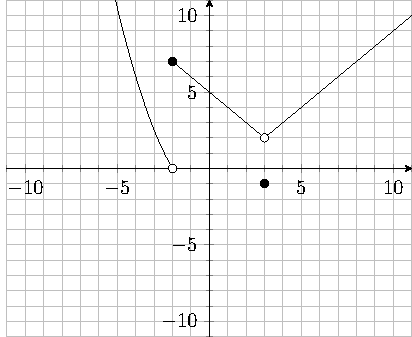
\includegraphics{finalgraph1.pdf}
\captionof{figure}{$f(x)$}\label{graph1exam1}%      only if needed  
\end{minipage}


\begin{questions}
\begin{multiplechoice}{5}
%8.5,8.6

\question According to the graph of $f(x)$, the $\lim_{x\to 3}f(x) $ equals which of the following.
\begin{answers}{3}
\ans $8$
\ans $2$
\ans $-1$
\ans $-3$
\ans The limit does not exist.
\end{answers}

%\textbf{Solution: d}


\question According to the graph of $f(x)$, the $\lim_{x\to -2^-}f(x) $ equals which of the following.
\begin{answers}{3}
\ans $7$
\ans $0$
\ans $-2$
\ans $-5$
\ans The limit does not exist.
\end{answers}

%\textbf{Solution: a}\\

\question According to the graph of $f(x)$, the $\lim_{x\to 5}f(x) $ equals which of the following.
\begin{answers}{3}
\ans $8$
\ans $4$
\ans $0$
\ans $-1$
\ans The limit does not exist.
\end{answers}

%\textbf{Solution: b}\\




\question According to the graph of $f(x)$, the function $f(x)$ is not continuous at $x=3$ because
\begin{answers}{3}
\ans $f(x)$ is not defined at $x=6$.
\ans there is a removable discontinuity at $x=6$
\ans $\lim_{x\to 6}f(x)$ does not exist.
\ans there is a horizontal asymptote at $x=6$. 
\ans there is a vertical asymptote at $x=6$.
\end{answers}

%\textbf{Solution: e}

%11.1,2

\nextpage

\question The graph of $g(x)$ is given below.\\

\begin{minipage}{\linewidth}% to keep image and caption on one page
\centering
\makebox[\linewidth]{}
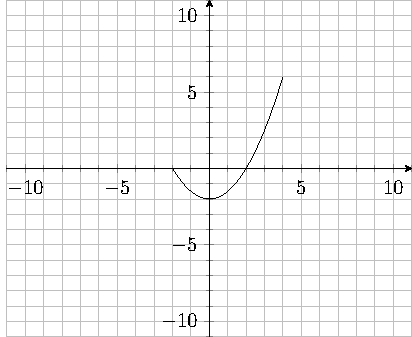
\includegraphics{exam1graph2.pdf}
\captionof{figure}{$g(x)$}\label{graph2exam1}%      only if needed  
\end{minipage}
According to the graph above, the domain and range of $g(x)$ are
\begin{answers}{2}
\ans Domain: $[-4,4]$, Range: $[-4,2]$
\ans Domain: $[-6,4]$, Range: $[-2,6]$
\ans Domain: $[-6,2]$, Range: $[-2,4]$
\ans Domain: $[-4,4]$, Range: $[-6,2]$
\ans Domain: $[-2,-6]$, Range: $[-2,4]$
\end{answers}
% Answer: 232/99

\question Find the domain of $f(x) = \frac{1}{x^2 - 16}$.
\begin{answers}{2}
\ans $(-2,2) \cup (2, \infty)$
\ans $(-\infty, -4) \cup (-4,4) \cup (4, \infty) $
\ans  $(-\infty, -4) \cup (0, \infty)$
\ans  $(-\infty, -2) \cup (-2,2) \cup (2, \infty)$
\ans $[-2,2)$
\end{answers}


\question Let $f(x) = \sqrt{4-x^2}$ and $g(x)=\ln(x)$.  What is the domain of $f(x)*g(x)$?
\begin{answers}{2}
\ans $(0,2]$
\ans $[-1,2)$
\ans $[-2,\infty)$
\ans $(0,\infty)$
\ans $[-2,2]$
\end{answers}

\nextpage

\question Given a function $f(x)$, then the graph of $2f\left(3 - x\right)$ will be
\begin{answers}{2}
\ans the graph of $f(x)$ shrunk horizontally by a factor of 2, shifted 4 units up, then reflected across the $x$-axis.
\ans the graph of $f(x)$ stretched vertically by a factor 3, shifted 2 units up, then reflected across the $y$-axis.
\ans the graph of $f(x)$ stretched vertically by a factor of 2, shifted 3 units to the right, then reflected across the $y$-axis.
\ans the graph of $f(x)$ stretched vertically by a factor of 2, shifted 3 units to the left, then reflected across the $y$-axis.
\ans the graph of $f(x)$ shrunk horizontally by a factor of 3, shifted 4 units to the right, then reflected across the $x$-axis.
\end{answers}


\question Jane notices that football game attendance is higher when the weather is warmer.  She finds that 100,000 fans attended a game when the temperature was $80^\circ$ and that 60,000 fans attended when the temperature was $40^\circ$.  Make a linear model that describes Jane's findings, where $t$ is the temperature in degrees and $F(t)$ is the number of fans attending a game.
\begin{answers}{3}
\ans $F(t) = 1000t+20,000$
\ans $F(t) = 1000t-40,000$
\ans $F(t) = 500t+30,000$
\ans $F(t) = 500t - 60,000$
\ans none of these
\end{answers}


\question A bacteria population doubles every 47 minutes.  If the initial population is 1000 bacteria, how many bacteria will there be after 5 hours?
\begin{answers}{3}
\ans $4.2 \times 10^4$
\ans $3.2 \times 10^3$
\ans $4.3 \times 10^3$
\ans $1.2 \times 10^3$
\ans $8.3 \times 10^3$
\end{answers}


%% EXAM 2


For the next two questions, use the following graph of $f'(x)$:\\


\begin{minipage}{\linewidth}% to keep image and caption on one page
\centering
\makebox[\linewidth]{}
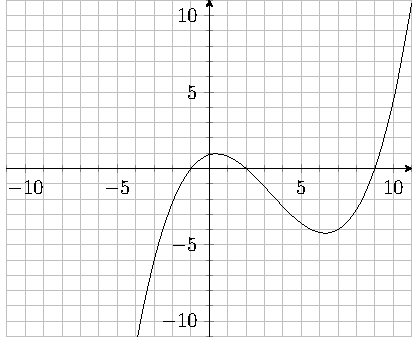
\includegraphics{exam2graph1.pdf}
\captionof{figure}{$f'(x)$}\label{graph1exam1}%      only if needed  
\end{minipage}


\question According to the graph of $f'(x)$, the original function $f(x)$ has a local maximum at
\begin{answers}{3}
\ans $-5$
\ans $-3$
\ans $0$
\ans $1$
\ans $5$
\end{answers}


\question According to the graph of $f'(x)$, the original function $f(x)$ is concave upward in which interval(s)?
\begin{answers}{2}
\ans $(-\infty, \infty)$
\ans $(-\infty, -3) \cup (1,5)$
\ans $(1, \infty)$
\ans $(-\infty, -3)$
\ans The original function $f(x)$ is never concave up.
\end{answers}


\question Find the derivative of the function $f(x) = \frac{3}{x^3} - 4x^2 + 3$.
\begin{answers}{2}
\ans $-\frac{15}{x^2} - 8x$
\ans $-\frac{15}{x^2} + 3$
\ans $-\frac{9}{x^4} -8x$
\ans $-\frac{9}{x^4} - 4$
\ans $-\frac{10}{x} - 3$
\end{answers}

\newpage

The graph of $g(x)$ is given below.\\

\begin{minipage}{\linewidth}% to keep image and caption on one page
\centering
\makebox[\linewidth]{}
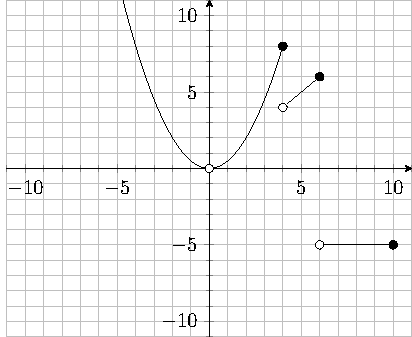
\includegraphics{exam2graph2.pdf}
\captionof{figure}{$g(x)$}\label{graph2exam1}%      only if needed  
\end{minipage}
\question According to the graph above, calculate the derivative of $g(x)$ at $x = 5$
\begin{answers}{2}
\ans $-\infty$
\ans -1.75
\ans 0
\ans 1
\ans The derivative does not exist at $x=5$.
\end{answers}

\question According to the graph above, estimate the derivative of $g(x)$ at $x = -2$
\begin{answers}{2}
\ans $-\infty$
\ans -1.75
\ans 0
\ans 1
\ans The derivative does not exist at $x= -2$.
\end{answers}


\question A vertical spring is released at time $t = 0$ seconds and begins to oscillate in a straight vertical line.
The height of its endpoint above the ground in meters is given by the function
$$h(t) = 5 - 0.1\cos(5t)$$
To two decimal places, what is the velocity (in meters/second) of the spring's endpoint at time $t = 3$ ?
\begin{answers}{2}
\ans 0.28
\ans 0.13
\ans 0.33
\ans 5.00
\ans 0.46
\end{answers}

\newpage

\question Find the linear approximation to $(3x-5)^4$ at $x = 2$
\begin{answers}{2}
\ans $3x - 5$
\ans $12x - 23$
\ans $12x + 25$
\ans $-4x - 7$
\ans $-4x + 8$
\end{answers}


\question We are given an unknown function $f(x)$ such that $f'(3) = 0$, $f'(x) < 0$ for all $x > 3$, and $f'(x) > 0$ for all $x < 3$.
We can conclude that at $x = 3$, the function $f(x)$ has 
\begin{answers}{3}
\ans a local min.
\ans a local max.
\ans an inflection point.
\ans an undefined derivative.
\ans positive $y$-value.
\end{answers}

\question Calculate the equation of the tangent line to $y = 6 \sqrt{x} - 3$ at $x = 9$
\begin{answers}{2}
\ans $y = -2x + 5$
\ans $y = 3x + 25$
\ans $y = x + 6$
\ans $y = -2x -4$
\ans $y = 3x - 25$
\end{answers}


\question Find the derivative of the function $\displaystyle f(x) = \frac{3}{x^2 +1}$.
\begin{answers}{2}
\ans $ \displaystyle \frac{6}{x^2 + 1}$
\ans $ \displaystyle  \frac{3 - 2x }{(x^2 + 1)^2}$
\ans $ \displaystyle -\frac{6x}{(x^2 + 1)^2}$
\ans $ \displaystyle  - \frac{3}{2x}$
\ans $ \displaystyle  \frac{3}{2x}$
\end{answers}

\question Find the derivative of the function $\ln(\sec(x^2 e^x))$.
\begin{answers}{2}
\ans $(2x + x^2)e^x \tan(x^2 e^x)$
\ans $\tan(x^2 e^x)$
\ans $ \sec(x^2 e^x)\tan(x^2 e^x)$
\ans $(2x + x^2)e^x \sec(x^2 e^x)\tan(x^2 e^x)$
\ans $2x^2e^x \tan(x^2 e^x)$
\end{answers}


%% EXAM 3


\question Find the absolute maximum and minimum values for the function 
$f(x) = 3x^2 - 6x + 4$ on the interval $[-1, 3]$
\begin{answers}{1}
\ans maximum value $= 1$, minimum value $ = -1$
\ans maximum value $= 10$, minimum value $ = -1$
\ans maximum value $= 13$, minimum value $ = 1$
\ans maximum value $= 10$, minimum value $ = 1$
\ans maximum value $= 13$, minimum value $ = -1$
\end{answers}


\question If $f'(x) = \frac{1}{\sqrt{x}} + 3x^2$ and $f(4) = 38$
\begin{answers}{2}
\ans $f(x) = \sqrt{x} + 3x^3 -30$
\ans $f(x) = 2\sqrt{x} + x^3 - 30$
\ans $f(x) = 2\sqrt{x} + x^3 + 30$
\ans $f(x) = \frac{2}{3} x^{3/2} + x^3 + 38$
\ans $f(x) = \frac{2}{3} x^{3/2} + x^3 - 30$ 
\end{answers}


\question A particle moves along a wire with velocity $v(t) = \sin(t) + 3$.  Find the
net change in position between times $t = 0$ and $t = \pi$
\begin{answers}{2}
\ans $1  + 3\pi$
\ans $-2 + 3\pi$
\ans $2 + 3\pi$
\ans $0$
\ans $3\pi$
\end{answers}

\question Calculate the indefinite integral 
$\displaystyle \int \frac{4}{x} + \sec^2(3x) \, dx$
\begin{answers}{2}
\ans $\frac{2}{x^2} + \frac{1}{3}\tan(3x) + C$
\ans $4 + 3 \tan(3x) + C$
\ans $4 \ln|x|  + \tan(3x) + C$
\ans $4  + \frac{1}{3}\tan(3x) + C$
\ans $4 \ln |x| + \frac{1}{3}\tan(3x) + C$
\end{answers}


\newpage

\question Use the fundamental theorem of calculus to find the derivative of 
$\displaystyle f(x) = \int_1^{x^2} \sin(\cos(t)) \, dt$
\begin{answers}{2}
\ans $\sin(\cos(x^2))$
\ans $x^2 \sin(\cos(x^2))$
\ans $(x^2 - 1) \sin(\cos(x^2))$
\ans $2x \sin(\cos(x^2))$
\ans $(2x - 1) \sin(\cos(x)$
\end{answers}

\question Use the geometric shape of the graph to find the integral 
$\displaystyle \int_{-2}^2 f(x)$ where 
$$ f(x) = 
\begin{cases}
5, & x \le 0
\sqrt{4 - x^2}, & x > 0
\end{cases}
$$
\begin{answers}{2}
\ans $$
\ans $\frac{27}{2} + \frac{3}{4}\pi$
\ans $\frac{9}{2} + 3\pi$
\ans $\frac{27}{2} + \frac{9}{4}\pi$
\ans $\frac{27}{2} + 9\pi$
\end{answers}

\question The acceleration of a particle is given by $a(t) = 6t - 2$.  The position
of the particle at times $t = 0$ and $t = 1$ are $s(0) = 2$ and $s(1) = 5$, respectively.  
The position function for the particle is
\begin{answers}{2}
\ans $s(t) = 3t^2 - 2t + 2$
\ans $s(t) = 3t^2 - 2t + 4$
\ans $s(t) = t^3 - t^2 + 5t + 2$
\ans $s(t) = t^3 - t^2 + 3t + 2$
\ans $s(t) = t^3 - 2t + 4$
\end{answers}

\question Calculate $\int_1^{e^2} \frac{\ln(x)}{x} \, dx$.
\begin{answers}{2}
\ans $e^{-4} - 1$ 
\ans $2e^{-4} - 1$
\ans $2e^{-4}$
\ans $e^{-2}$
\ans $2$
\end{answers}

\question Calculate the area between the curves $y = x$ and $y = x^2$.
\begin{answers}{3}
\ans $\frac 1 3$ 
\ans $\frac 1 6$ 
\ans $\frac 2 3$ 
\ans $1$ 
\ans $- \frac 1 2$ 
\end{answers}

\question What is the average value of the function $f(x) = \sin(x)$ on $[0, \pi]$
\begin{answers}{3}
\ans $2$
\ans $-2\pi$
\ans $-\frac{\pi}{2}$
\ans $\pi$
\ans $\frac{2}{\pi}$
\end{answers}

\end{multiplechoice}
\end{questions}
\end{document}

*************************************************************************
*************************************************************************
